\section{DataTypeTemplates}

El elemento \emph{DataTypeTemplate} 
y todos 
sus elementos hijos ser�an 
lo m�s pr�ximo 
a definiciones de clase. 
Si bien sabemos que 
los archivos XML se utilizan 
generalemente como
mecanismo para la \gls{SO},
en realidad el \emph{DataTypeTemplate} 
es lo m�s cercano a la definici�n de 
clases del paradigma \gls{O-O-es}, 
pues los elementos hijos de
\emph{DataTypeTemplates} 
sirven como plantillas a trav�s 
del cual las instancias son creadas
en un IED. De hecho, tambi�n puede
relacionarse un \emph{DataTypeTemplate}
directamente con el modelo de 
informaci�n inicialmente ubicado 
en el elemento \emph{Substation}, 
pero considerando que el 
SCL XML Schema no define v�nculos 
obligatorios entre el elemento \emph{Substation}
y el elemento \emph{DataTypeTemplate}
(en el elemento \emph{IED} s� lo hace), 
entonces en este trabajo se opt� por 
vincular directamente el \emph{DataTypeTemplate}
con el elemento \emph{IED} de 
cada \gls{ICD}. 
En la figuras 
\ref{fig:SCL-DataTypeTemplates-depthMax-conHerencia}
y
\ref{fig:SCL-DataTypeTemplates-depthMax-heredado}
se pueden observar los diagramas 
de clases del DataTypeTemplate.
Los mismos diagramas, en forma simplificada,
son proveidos en las figuras
\ref{fig:SCL-DataTypeTemplates-depthMax-conHerencia-simplificado}
y 
\ref{fig:SCL-DataTypeTemplates-depthMax-heredado-simplificado}.

\begin{figure}
\begin{center}
  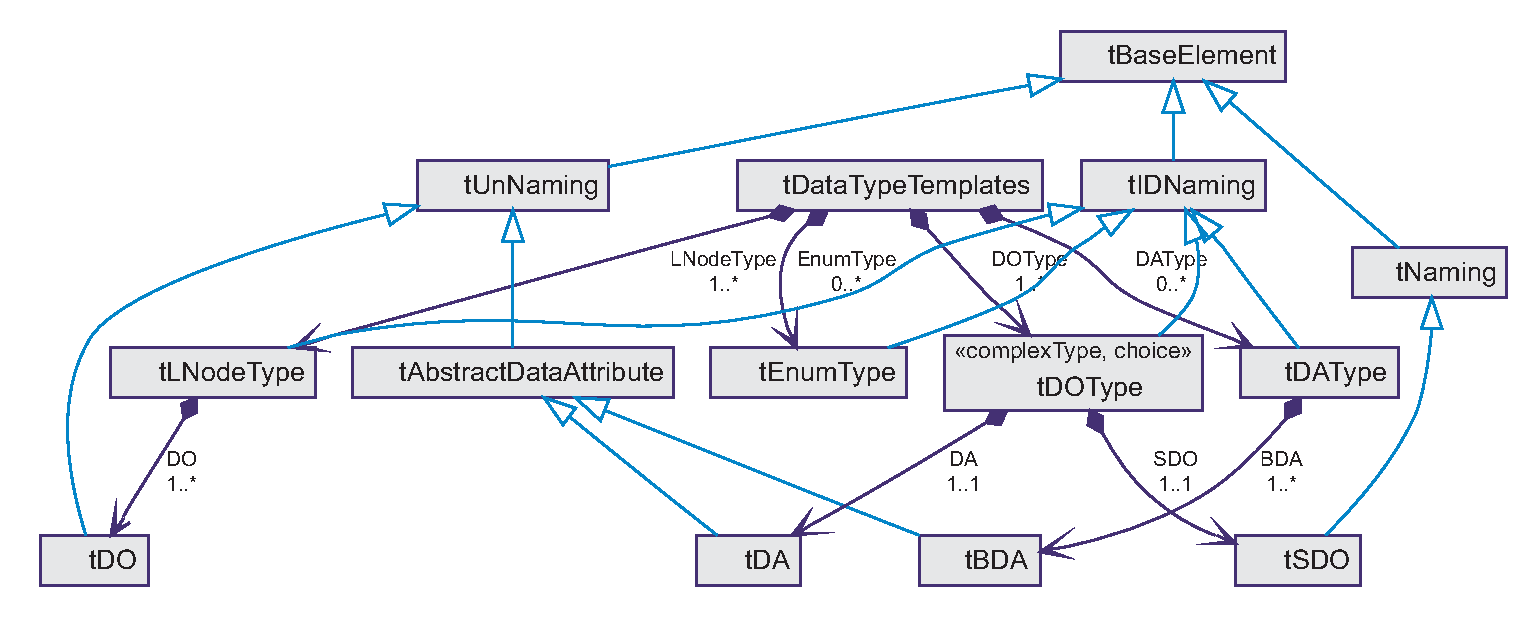
\includegraphics[width=1.0\linewidth]{chapters/enfoque/figures/scl-DataTypeTemplates-depthMax-conHerencia-simplificado.eps} 
  \caption{Diagrama de clases simplificado del elemento \emph{DataTypeTemplate}
  del SCL, incluyendo sus clases abstractas}
  \label{fig:SCL-DataTypeTemplates-depthMax-conHerencia-simplificado}
\end{center}
\end{figure}

\begin{figure}
\begin{center}
  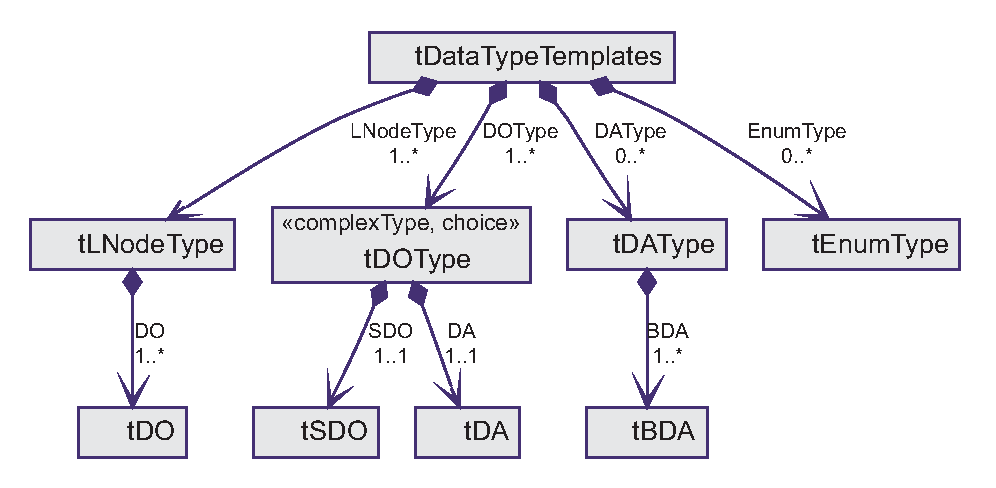
\includegraphics[width=0.7\linewidth]{chapters/enfoque/figures/scl-DataTypeTemplates-depthMax-heredado-simplificado.eps} 
  \caption{Diagrama de clases simplificado del elemento \emph{DataTypeTemplate}
  del SCL, omitiendo sus clases abstractas}
  \label{fig:SCL-DataTypeTemplates-depthMax-heredado-simplificado}
\end{center}
\end{figure}


\begin{landscape}
\thispagestyle{empty}
\begin{figure}
\begin{center}
  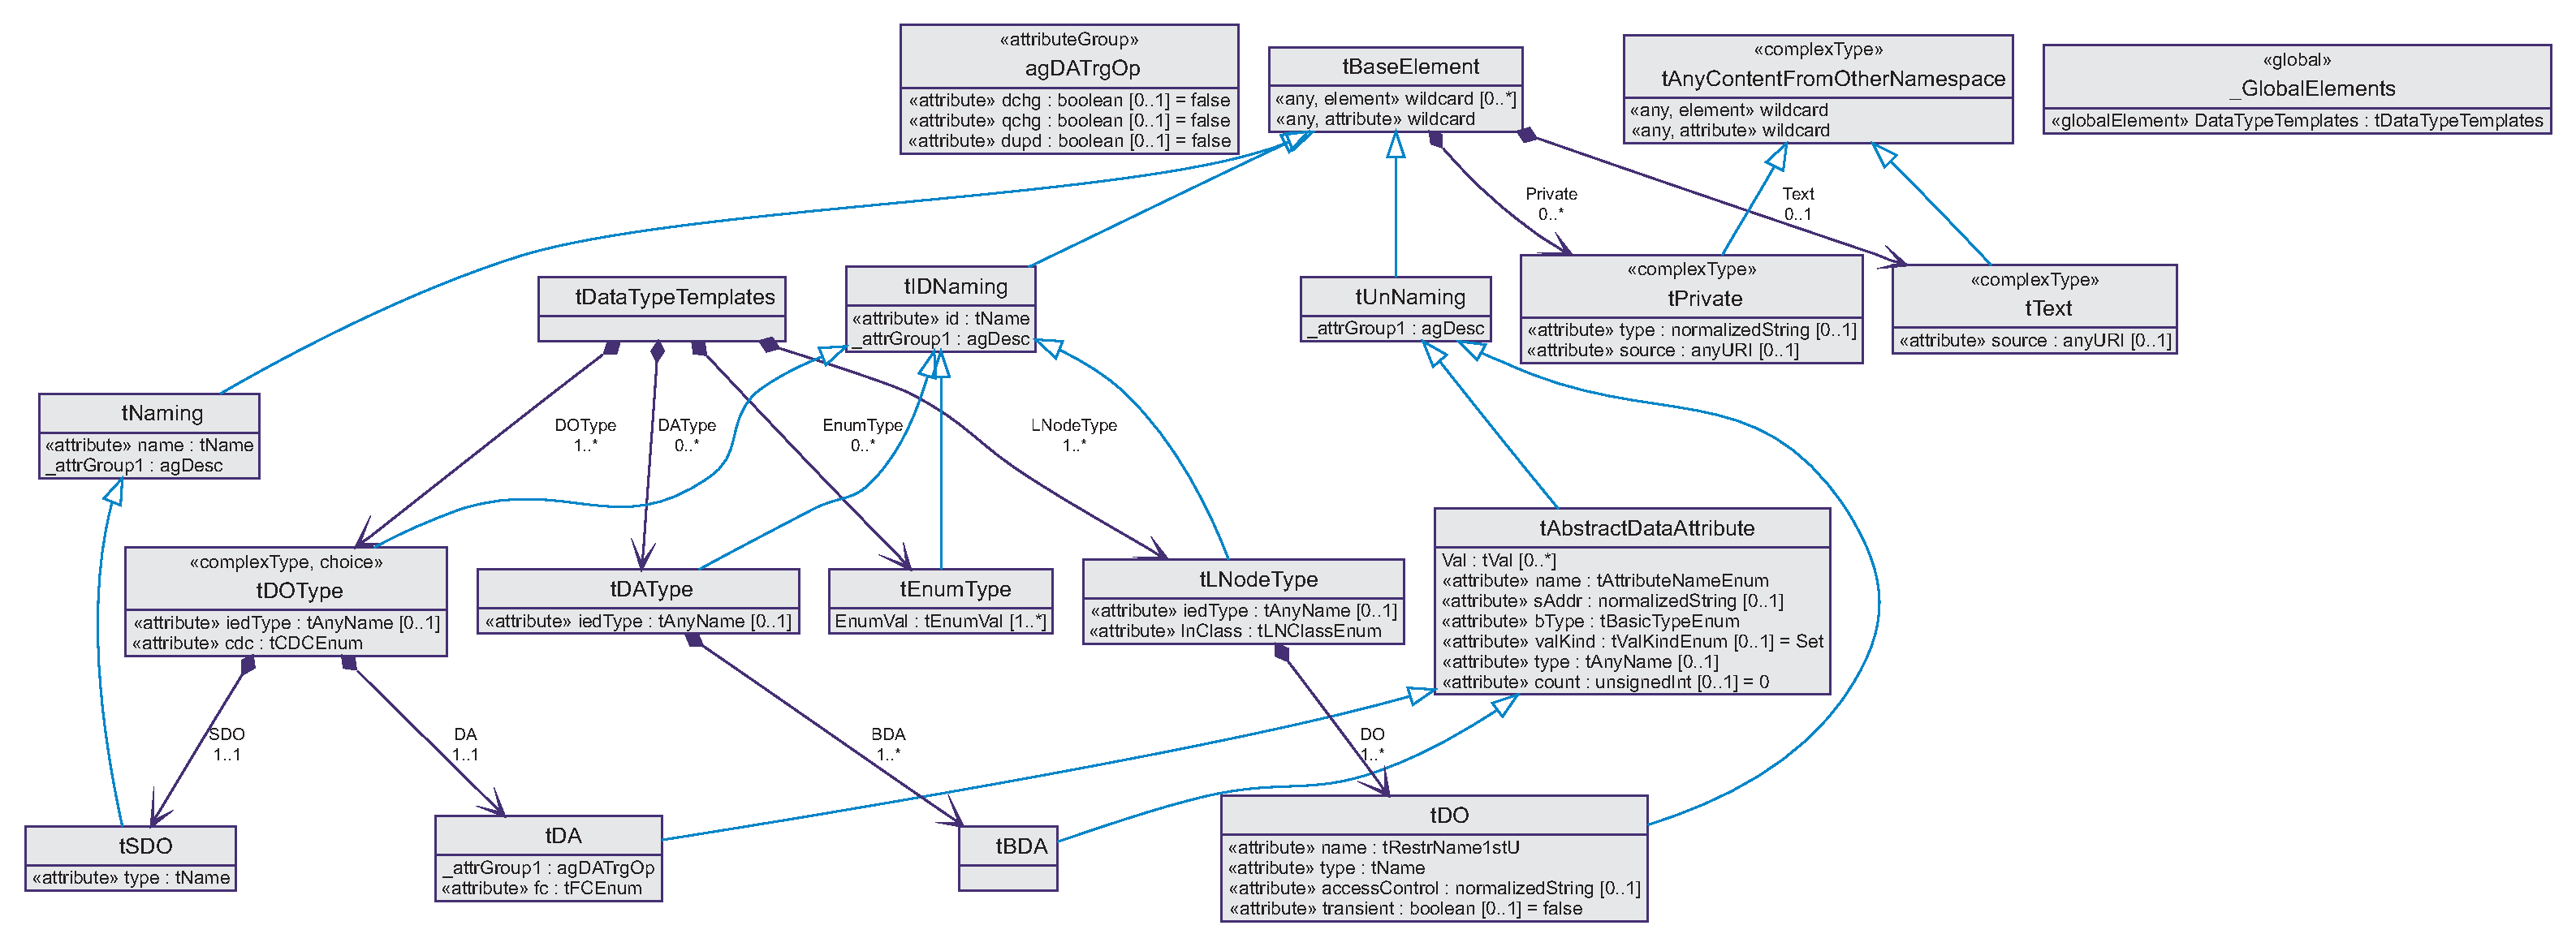
\includegraphics[width=1.0\linewidth]{chapters/enfoque/figures/scl-DataTypeTemplates-depthMax-conHerencia.eps} 
  \captionsetup{font=scriptsize}
  \caption{Clases del elemento \emph{DataTypeTemplate} del SCL, incluyendo
  sus clases abstractas}
  \label{fig:SCL-DataTypeTemplates-depthMax-conHerencia}
\end{center}
\end{figure}
\end{landscape}


\begin{landscape}
\thispagestyle{empty}
\begin{figure}
\begin{center}
  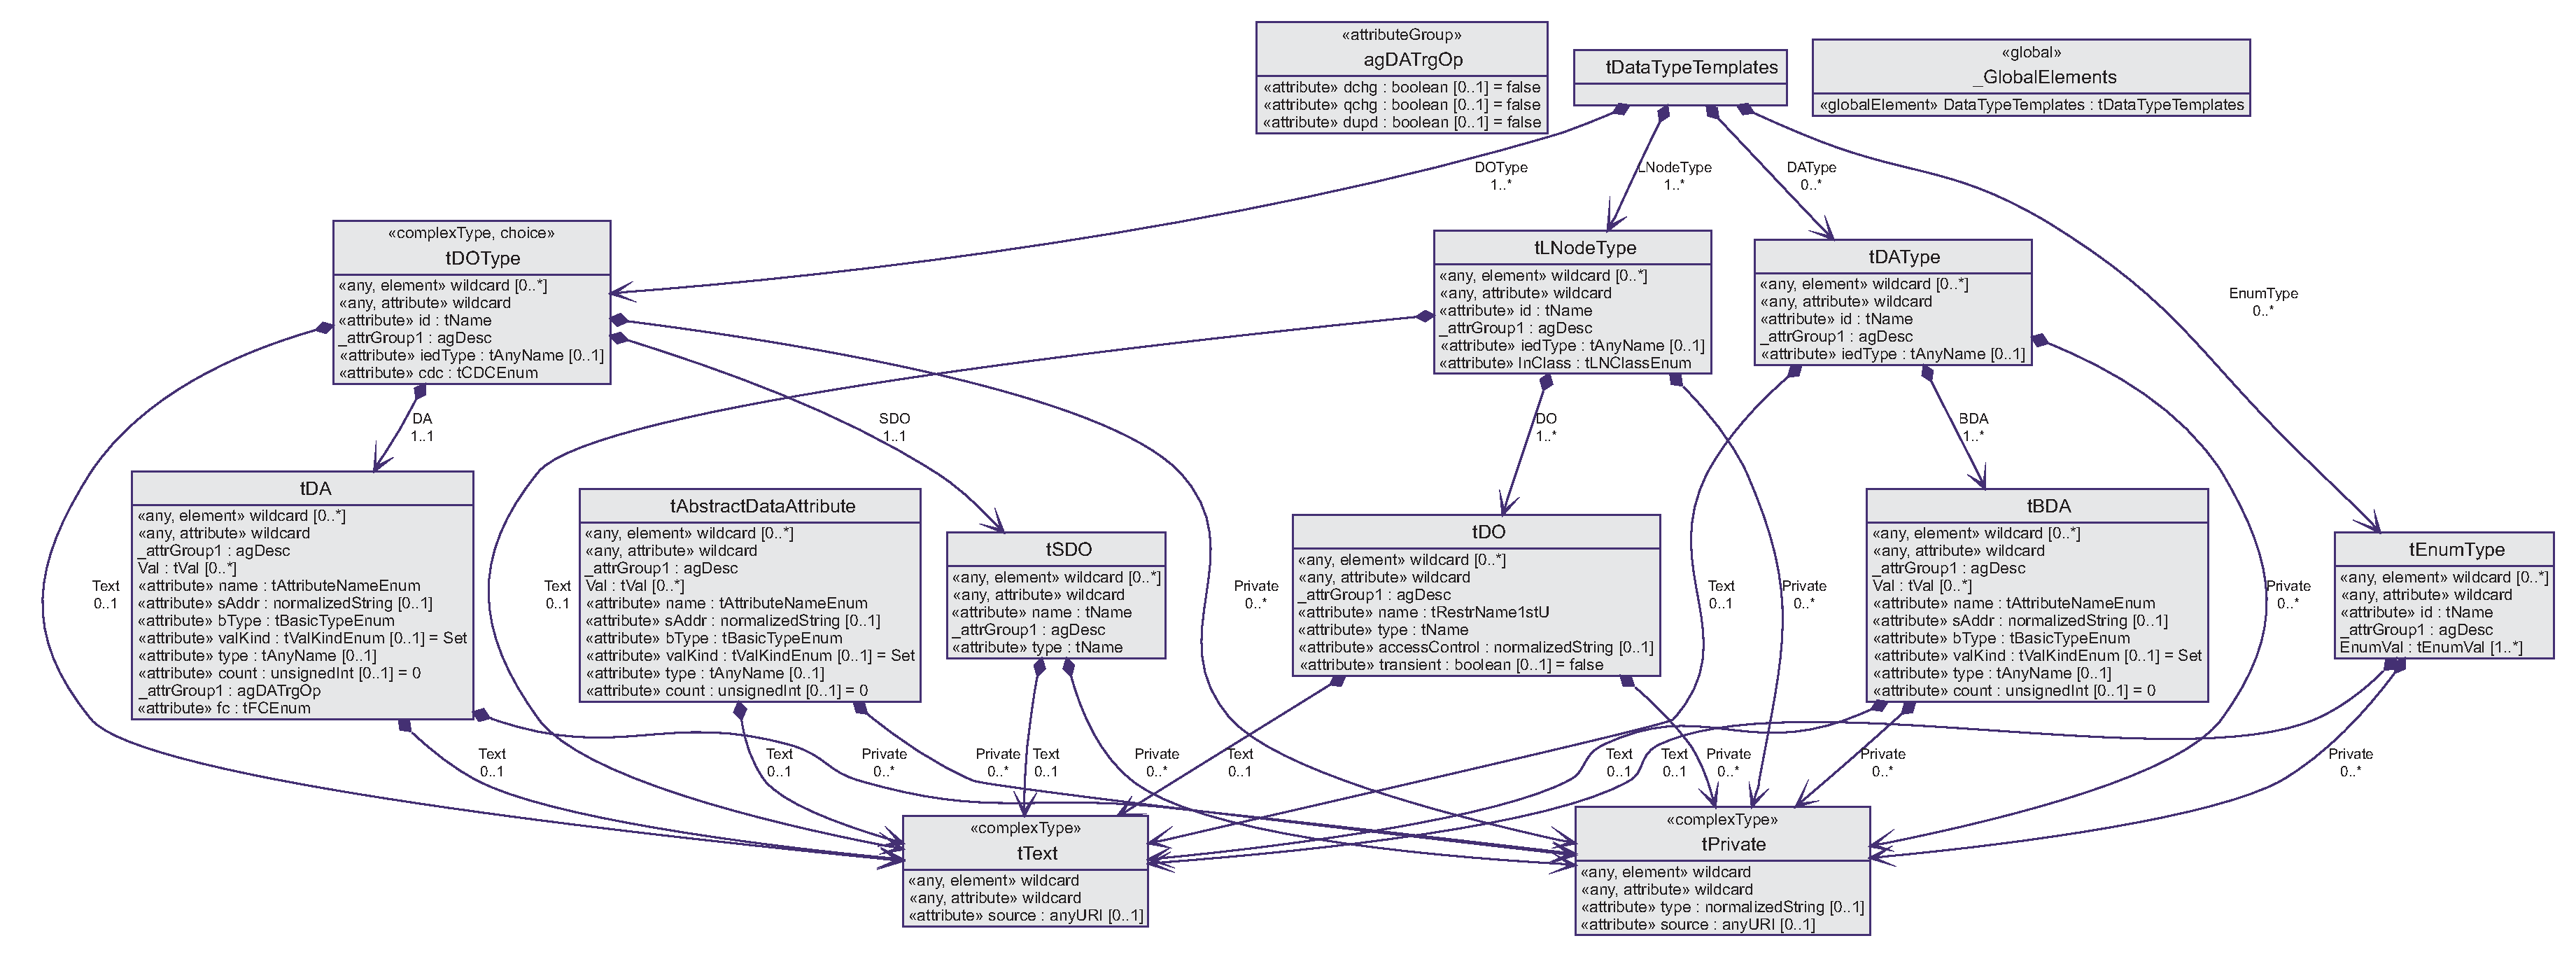
\includegraphics[width=1.0\linewidth]{chapters/enfoque/figures/scl-DataTypeTemplates-depthMax-heredado.eps} 
  \captionsetup{font=scriptsize}
  \caption{Clases del elemento \emph{DataTypeTemplate}
  del SCL, omitiendo sus clases abstractas}
  \label{fig:SCL-DataTypeTemplates-depthMax-heredado}
\end{center}
\end{figure}
\end{landscape}


Seg�n las directrices del EPRI \cite{Epri:2004}, 
uno de los primeros pasos del proceso de ingenier�a 
para la 
especificaci�n de sistemas de 
automatizaci�n de subestaciones usando la norma IEC 61850
consiste en identificar los datos
disponibles, y en base a estos datos, determinar 
los nodos l�gicos correspondientes.

En el presente trabajo se realiz� este paso 
escribiendo en el elemento \textbf{DataTypeTemplate}
de un s�lo archivo SCL todos los nodos l�gicos 
seg�n los datos identificados del sistema. 
En este paso, a�n no se ubican los nodos l�gicos
en los dispositivos l�gicos ni f�sicos. 


